\documentclass[12pt, twoside]{report}

% Packages for equations and math symbols
\usepackage{amsmath}
\usepackage{amsfonts}
\usepackage{amssymb}

% Packages for figures
\usepackage{graphicx}
\usepackage{caption}
\usepackage{subcaption}
\usepackage{float}

% Packages for code
\usepackage{listings}
\usepackage{xcolor}

\definecolor{codegreen}{rgb}{0.1,0.6,0.1}
\definecolor{codegray}{rgb}{0.3,0.3,0.3}
\definecolor{codepurple}{rgb}{0.68,0,0.82}
\definecolor{backcolour}{rgb}{0.94,0.95,0.95}

% Python
\lstdefinestyle{python}{
    language=Python,
    backgroundcolor=\color{backcolour},
    commentstyle=\color{codegreen},
    keywordstyle=\color{magenta},
    numberstyle=\tiny\color{codegray},
    stringstyle=\color{codepurple},
    basicstyle=\linespread{1.0}\ttfamily\footnotesize,
    breakatwhitespace=false,
    breaklines=true,
    captionpos=b,
    keepspaces=true,
    numbers=left,
    numbersep=5pt,
    showspaces=false,
    showstringspaces=false,
    showtabs=false,
    tabsize=2,
}

\lstdefinestyle{inlinepython}{
    language=Python,
    basicstyle=\ttfamily\small,
    commentstyle=\color{codegreen},
    keywordstyle=\color{magenta},
    stringstyle=\color{codepurple},
    showstringspaces=false,
}

% Pseudocode
\lstdefinelanguage{Pseudocode}{
  morekeywords={for, to, end, if, then, else, while, do, repeat, until, return},
  morecomment=[l]{\#},
  morestring=[b]',
  sensitive=true
}
\lstdefinestyle{pseudocode}{
    language=Pseudocode,
    basicstyle=\ttfamily,
    keywordstyle=\bfseries,
    commentstyle=\itshape,
    xleftmargin=2em,
    aboveskip=1em,
    belowskip=1em,
}

% \lstset{style=mystyle}

% Double spacing
\usepackage{setspace}
\doublespacing

% Times New Roman font
\usepackage{times}

% Page margins
\usepackage[margin=1in]{geometry}

\begin{document}

% Title page
\title{CS 8770 \\ Neural Networks \\ Project 1}
\author{Drew Dahlquist \\ dgdtx5}
\date{March 2, 2023}
\maketitle

% Table of contents
\tableofcontents

% List of figures and tables (optional)
% \listoffigures
% \listoftables

% Chapter 1: Introduction
% \chapter{Introduction}

% Chapter 2: Technical Description
\chapter{Technical Description}

\section{Introduction}
My goals for this project were to familiarize myself with the nuances of implementating the
various networks as well as better understanding the ``art'' of training them.
Personally, I have a strong background in mathematics and statistics, so I wanted to use this
project as an oppurtunity to explore the more practical issues around neural networks instead 
of dwelling on the underlying mathematical/statistical theory that I'm already familiar with.

\section{Data}

The datasets used for this project were MNIST, samples of which can be seen in the
below figure taken from Wikipedia, and FashionMNIST which is similar except consists of
``fashion'' items instead of hand written digits.
Both datasets contain 60,000 training examples and 10,000 testing examples, as well as 
10 total classes.
FashionMNIST is typically seen as being slightly more challenging than DigitMNIST, which
experimentally looks to be the case from later work in this project.
I was able to trian on the full 60,000 MnistExamples for each as well as test on the full
10,000 so was able to leave the datasets as is without down-sampling, etc.

\begin{figure}[H]
    \centering
    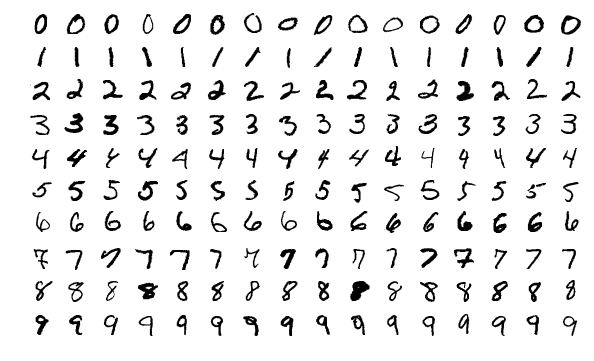
\includegraphics[width=0.65\textwidth]{figures/MnistExamples.png}
    \caption*{Example MNIST digits (source: wikipedia.com)}
\end{figure}

In order to load the data as well as handle a lot of the overhead for
batching, shuffling during training, etc. I used the torch datasets as well
as Dataloader's which I found to be really useful so I could keep my focus on 
working with the networks as opposed to boilerplate data management code.
A similar code chunk can also be used for FashionMNIST

\begin{lstlisting}[style=Python,caption=Loading MNIST,label=lst:python]
from torchvision import datasets
from torchvision.transforms import ToTensor
from torch.utils.data import DataLoader

train_data = datasets.MNIST(
root='data',
train=True,
download=True,
transform=ToTensor())

test_data = datasets.MNIST(
    root='data',
    train=False,
    download=True,
    transform=ToTensor())

batch_size = 4
train_dl = DataLoader(train_data, batch_size=batch_size, shuffle=True)
test_dl = DataLoader(test_data, batch_size=batch_size, shuffle=True)
\end{lstlisting}

\section{Networks}

\subsection{Multi-Layer Perceptron}

A Multi-Layer Perceptron is a fairly simple yet very important model of a neural network.
At a high-level, it consists of many individual ``perceptrons'' organized into various layers
which are highly ``connected'' to the other neurons in the previous and subsequential layers, but
typically not the same layer or any others. A single perceptron is an abstraction for a mathematical 
function which aggregates it's input, possibly applies a bias term, and runs that value through an
activation function such as ReLU, which is what I typically used throughout this project and is given below.

\begin{figure}[H]
    \centering
    \begin{align}
        \varphi(x) = \begin{cases} 
            0 & x < 0 \\
            x & 0 \leq x
        \end{cases}
    \end{align}
    \caption*{ReLU Activation Function}
\end{figure}

A connection between neurons simply means that the output of one neuron is passed to the input of the next
it's connected to, and is typically assigned a weight in order to characterize how much influence the value
should have. Mathematically, this all wraps up nicely into a (possibly) large composition of matrix 
mulitplications (linear) and applications of activiation functions (non-linear) which is written out
below.

\begin{figure}[H]
    \centering
    \begin{align}
        N(x) = W^l \cdots \varphi(W^{l-1} \varphi(W^2\varphi(W^1(x))))
    \end{align}
    \caption*{MLP mathematically}
\end{figure}

For my implementation of MLP's, I stuck to using the ReLU activation function most of the time,
although I did try some others, as they all appeared to give the same results thus it didn't make much
sense to me worrying about what was being used for this project. The main feature I was interested in was
the amount/size of the various layers within the network, which I talk more about in the results section.

\subsection{Radial Basis Function Network}

I found Radial Basis Function (RBF) Networks to be the most odd of the three I spent time investigating.
They proved to require much more care than the other networks and yet didn't feel like that extra effort
spent paid off much at all – at least for the datasets used. Roughly speaking, RBF Nets pass data through
a layer of neurons each endowed with a Radial Basis Function of their own, composed with a linear layer
to pare down the feature space to make a final output. The RBF Layer, in theory, must capture all the 
non-linearity within the given problem, as the linear layer will only make linear combinations of the 
RBF Layer's resulting features (linear is in the name afterall). The nature of the functions I used, and 
which are probably typically used, as basis function aim to only capture local behavior, which was one 
of my main difficulties in working with this form of network.
The exact function I used throughout this project is given below.

\begin{figure}[H]
    \centering
    \begin{align}
        f_i(x) = \exp\left(-\frac{1}{2}\frac{||\mathbf{x}-\mathbf{\mu_i}||^2}{\sigma_i^2}\right)
    \end{align}
    \caption*{Example Gaussian Radial Basis Function}
\end{figure}

While I was developing my RBF Net I discovered they are particularly susceptible to the curse of dimensionality.
Due to them being local function approximators and therefore needing to measure distances, when the 
dimensionality of the input is suitably large they severly struggle to learn.
This makes sense as high-dimensional Euclidean space gets incredibly sparse as the dimension increases causing
distance functions to lose their usefulness. In order to overcome this and get my network to learn
I forced all samples and $\mu$ vectors to have a unit norm to reign in this sparsity, which did the job, and
is discussed more in the experimental results section.

For my exact implementation, I only trained the final linear layer's weights, and left the $\mu$'s and
$\sigma$'s fixed while also only using a single $\sigma$ for each neuron and not a full $\Sigma$ since
experimentally this proved to be sufficient. Part of the reason for not learning the $\mu$'s and $\sigma$'s
was actually because I could not figure out what extra was needed in my torch code since by default the values
were not being updated.

\subsection{Convolutional Nerual Network}

Convolutional Neural Networks are a nice extension to MLPs that make them better suited for
image data. The key feature, and where they get their name from, is in using convolutional layers which
apply a set of learned filters to the input image. These filters tend to make use of the data locality in image
data to hopefully learn things like edges, corners, etc.
Another common layer that's typically added to CNNs is a pooling layer that reduces the the size of the image
by subsampling it and passing through (typically) the max value.
Lastly, CNNs tend to use dropout, which is a technique to help regularize neurel network by randomly
``turning off'' certain neurons during training which has the result of effectively training an ensemble of
more sparse networks.

The general structure of the CNNs I used in this project is a set of some convolutional layers followed
by a simple MLP at the end in order to make the final 10-class classification. I stuck with relatively simple
CNNs as I didn't think a deep network would be needed to solve these datasets and it would only make
my training times unnecessarily long.

\section{Training}

There are a few different methods for presenting training data to a network in order
for it to learn – batch, mini-batch, and sequential. The below equation provides all of these
as a special case – batch occurs when $B = N$, mini-batch when $1 < B < N$, and sequential $B = 1$.
For my project I mostly used mini-batch as this is what I'm aware of being most common and it also provides
for making some nice trade-offs between training quality and time.

\begin{figure}[H]
    \centering
    \begin{align}
        \mathcal{E}_{batch} = \frac{1}{2B} \sum_{n=1}^{B} \sum_{j=1}^{C} e_j^2(n) \\
        \Delta w_{ji} = - \eta \frac{\partial \mathcal{E}_{batch}}{\partial w_{ji}} = 
        - \frac{\eta}{B} \sum_{n=1}^{B} e_j(n)\frac{\partial e_j(n)}{\partial w_{ji}}
    \end{align}
    \caption*{Error equations}
\end{figure}

Using the above error equations we are primarily focused on estimating the gradient of the error
so we may use it in gradient-based optimization algorithms. One interesting thing to note as that
as we increase the mini-batch size, i.e., go from sequential learning to full blown batch learning, 
we are effectively obtaining ``estimates'' of the true error gradient. Going into this project
I would've guessed that using the full batch in order to obtain the true gradient of the error
would be ideal, since that provides the most information for us to use during optimization.
However, this approach is also more timely during training as between each optimization step we
spend more time on calculating gradients as opposed to actually minimizing our objective function, 
which is what we set out to do. This is something I focus more on during my experimentation and is 
discussed in later sections.

For all training/testing I used \lstinline[style=inlinepython]{nn.CrossEntropyLoss()}
as I felt it was most natural for doing multi-class classification.
The mathematical formulation for this is given as follows:

$\ell(x,y) = \{l_1, \ldots, l_B\}^T$ where $l_i$ is defined as 

\[
    l_i := -\log \frac{\exp(x_{i,y_i})}{\sum_{c=1}^{C} \exp(x_{i,c})}
\]

I made use of several optimization algorithms which I formulate below.
I did not use many of the extra hyperparameters for most of the algorithms such as 
momentum or weight decay in order to have more time to allocate to other algorithms instead
of spending a lot of time focusing on just one.
For simplicity we define $g_t := \nabla_{\theta} f_t(\theta_{t-1})$ as the gradient, and
$\gamma$ for the learning rate.
Stochastic gradient descent (SGD) is the simplest algorithm I used, where the update rule
is given below.

\begin{figure}[H]
    \centering
    \begin{align}
        \theta_t &= \theta_{t-1} - \gamma g_t
    \end{align}
    \caption*{SGD update equations}
\end{figure}

The ``middle ground'' of optimization algorithms I used was Adagrad. Adagrad makes use of a slightly
more sophisticated update rule than SGD, which is given below, and – informally – attempts to adapt
the learning rate using second-order curvature information about each parameter to improve upon the 
simple $\gamma$ in SGD. I've written the update rule in a way that emphasizes this relation to SGD.

\begin{figure}[H]
    \centering
    \begin{align}
        \textit{state\_sum}_t &= \textit{state\_sum}_{t-1} + g_t^2 \\
        \theta_t &= \theta_{t-1} - \frac{\gamma}{\sqrt{\textit{state\_sum}_t} + \epsilon} g_t
    \end{align}
    \caption*{Adagrad update equations}
\end{figure}

Lastly, the most sophisticated algorithm I tested was Adam. Again, the parameter update rule is
essentially the same as SGD, but Adam does a lot of auxillarly computation in hopes to provide
the optimal step size.

\begin{figure}[H]
    \centering
    \begin{align}
        m_t &= \beta_1 m_{t-1} + (1-\beta_1)g_t \\
        v_t &= \beta_2 v_{t-1} + (1-\beta_2)g_t^2 \\
        \widehat{m_t} &= m_t / (1-\beta_1^t) \\
        \widehat{v_t} &= v_t / (1-\beta_2^t) \\
        \theta_t &= \theta_{t-1} - \gamma \widehat{m_t} / (\sqrt{\widehat{v_t}}+\epsilon)
    \end{align}
    \caption*{Adam update equations}
\end{figure}

% Chapter 3: Experiments and Results
\chapter{Experiments and Results}

\section{Playing with Various Hyperparameters}

\subsection{Batch Size}

In order to explore the effect of varying batch size on the various aspects of training a network
(train loss, test loss, real-time taken to train, etc.) I used a CNN with a single convolutional layer
followed by a small MLP with one hidden layer resulting in 101,146 total trainable parameters.
The model statement is given in Listing 3.1.
The optimizer was \lstinline[style=inlinepython]{optim.SGD()} with a learning rate of 1e-3 and 
was run for 5 epochs on a fresh network for each batch size.
I focused on the DigitMNIST dataset and trained the same CNN as described above on batches of 
1, 4, 16, 64, and 128 using the full 60,000 training points.

\begin{lstlisting}[style=Python,caption=CNN Model,label=lst:python]
CNN(
    (flatten): Flatten(start_dim=1, end_dim=-1)
    (conv): Sequential(
        (0): Conv2d(1, 8, kernel_size=(3, 3), stride=(1, 1), padding=(1, 1))
        (1): ReLU(inplace=True)
        (2): MaxPool2d(kernel_size=2, stride=2, padding=0, dilation=1, ceil_mode=False)
        (3): Dropout(p=0.2, inplace=False)
    )
    (mlp): Sequential(
        (0): Linear(in_features=1568, out_features=64, bias=True)
        (1): ReLU(inplace=True)
        (2): Dropout(p=0.2, inplace=False)
        (3): Linear(in_features=64, out_features=10, bias=True)
    )
)
\end{lstlisting}

The results of this experiment are summarized in Table 3.1.
I was very surprised to see that the training quality actually decreased as batch size increased, 
as I was expecting the opposite. I figured that a larger batch size giving
a better estimate of the true gradient would result in the network learning both better and faster, but 
experimentally this doesn't look to be the case, at least for this complexity of network and dataset.
Although my intuition didn't hold for this particular experiment, I'm left wondering if there is some
combination of optimizer, parameter count, dataset, etc. where it is the case that an increased batch size
results in more effective training.

\begin{table}[h]
    \centering
    \begin{tabular}{|c|c|c|c|}
    \hline
     Batch Size & Avg. Train Loss & Test Loss & Avg. Epoch Time \\
    \hline
    1 & 4.1e-3 & 0.0550 & 60s \\
    \hline
    4 & 0.1447 & 0.1010 & 30s \\
    \hline
    16 & 0.3575 & 0.3733 & 20s \\
    \hline
    64 & 0.8317 & 0.6988 & 12s \\
    \hline
    128 & 1.9468 & 1.7143 & 5s \\
    \hline
    \end{tabular}
    \caption{Batch size influence on model performance}
\end{table}

I decided not to dwell too long on invistigating the effects of batch size for every circumstance
and instead moved on to testing out other considerations such as learning rate, various layer structures,
and the results of more optimization algorithms. However, I decided to use what I learned from these
quick batch size experiments to better influence those tests. Moving forward I wound up mostly keeping a 
batch size in the 1 to 8 range in order to compromise on training effectiveness as well as my iteration 
times between various tests.

\subsection{Learning Rate}

In addition to varying the batch size, I also wanted to quickly get a better 
intuiton for how the learning rate affects training.
To test the effects of different learning rates on network training 
I used an MLP with 3 hidden layers of sizes 512, 256, 128.
I stuck with a simple optim.SGD() in order to not tarnish my tested learning rates
with those that more advanced optimization algorithms take it upon themselves to calculate.
I used a batch size of 8 and trained each network for 15 total epochs each, 
in order to maintain some training quality as mentioned in the previous
section while still being able to iterate on my testing. I also used FashionMNIST as I wanted the data
to be difficult enough to learn to hopefully magnify any differences among different learning rates.

The below few plot show the training $log$ loss versus training iteration of a few different 
learning rate schemes, roughly going from worst (top) to best (bottom).
All are within a ``reasonable'' range for learning rate, as any value either too small or too large
simply results in little to no learning and isn't all that interesting.
range for learning rate,
The main thing to look at is the y-axis values and scale, as all of the plots result from training 
for 15 epochs all with the same batch size each time.

\begin{figure}[H]
    \centering
    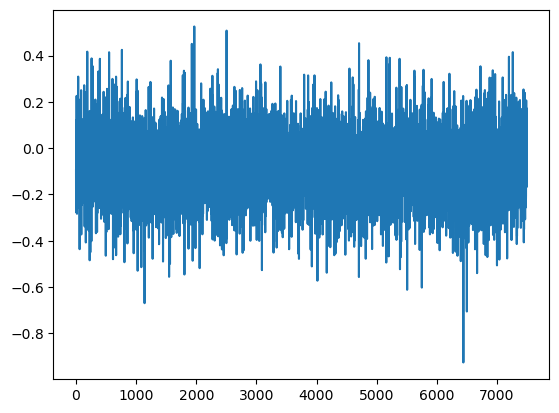
\includegraphics[width=0.65\textwidth]{figures/1e-4.png}
    \caption*{learning\_rate = 1e-4}
\end{figure}

\begin{figure}[H]
    \centering
    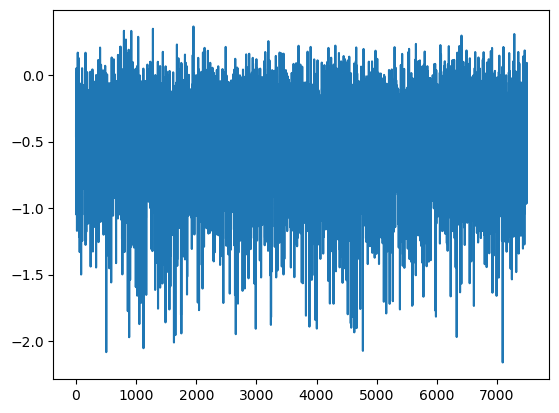
\includegraphics[width=0.65\textwidth]{figures/1e-3.png}
    \caption*{learning\_rate = 1e-3}
\end{figure}

\begin{figure}[H]
    \centering
    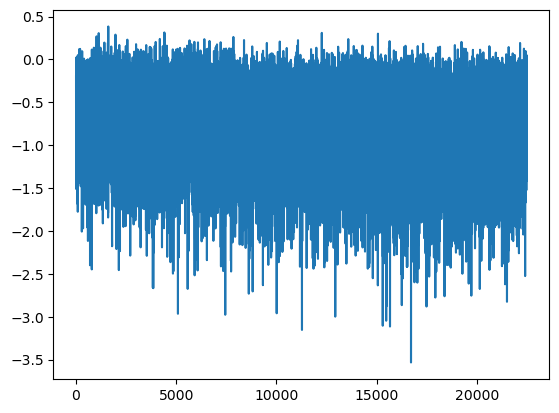
\includegraphics[width=0.65\textwidth]{figures/1e-234.png}
    \caption*{learning\_rate = 1e-2, 1e-3, 1e-4}
\end{figure}

From the plots it looks like the best way to train for this specific instance is to
begin with a ``large'' learining rate such as 1e-2, and slowly decrease it as we go through training
since we are hopefully nearing convergence. I don't think, however, that these testing scenarios were
entirely approaching convergence within 15 epochs and could have probably been trained at a higher learning
rate for longer in order to truly obtain a good model, but that wasn't the goal here as I simply wanted to 
plot the change in loss for different learning rates.

\section{Networks}

\subsection{Multi-Layer Perceptron}

\begin{lstlisting}[style=Python,caption=MLP Class,label=lst:python]
class MLP(nn.Module):
    
    # H: list of hidden layer dims
    # phi: non-linearity to use
    # n_classes: num of classes to pred
    def __init__(self, H, phi=nn.ReLU(), n_classes=10):
        super(MLP, self).__init__()
        self.flatten = nn.Flatten()
        self.layers = nn.Sequential()
        # create hidden layers based off input list H
        H.insert(0,28*28) # input layer
        [self.layers.append(nn.Linear(h,l)).append(phi) for h, l in zip(H,H[1:])] # hidden layers
        self.layers.append(nn.Linear(H[-1],n_classes)) # output layer

    def forward(self, x):
        x = self.flatten(x)
        return self.layers(x)
\end{lstlisting}

Working with implementating an MLP was the most fun for me, mainly because it was enjoyable to see
just how much can be accomplished with some matrix mulitplications, simple non-linear functions, and
then some elementary calculus. Since the network structure of MLP's is also so simple, I was able to
easily code it up so all I had to specify was the number of neurons I want in each hidden layer and 
have Python/PyTorch take it from there which made further testing all the more enjoyable.

Possibly the most interesting experimental result I obtained from working with the MLP was
that a ``null'' MLP with no hidden layer what-so-ever – literally just a $10 \times 784$ matrix multiplication –
was able to achieve incredible performance on both DigitMNIST and FashionMNIST as shown in the 
confusion maticies below. Furthermore, this was achieved using nothing fancy to train – simple SGD,
a fixed 1e-3 learning rate, and range for 5 epochs.

% MLP, no hidden layer, trained for 5 epochs with SGD on Digit
\begin{figure}[H]
    \centering
    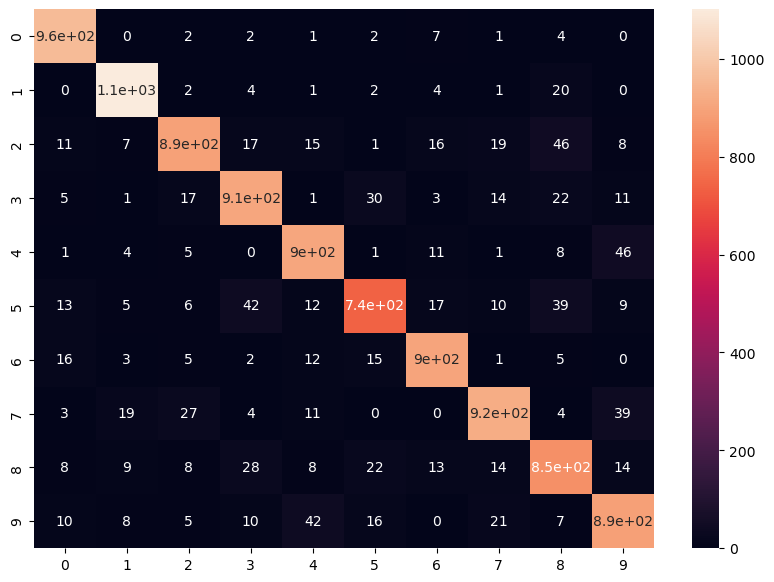
\includegraphics[width=0.65\textwidth]{figures/mlp_no_hidden_cf.png}
    \caption*{MLP with no hidden layer on DigitMNIST}
\end{figure}

% MLP, no hidden layer, trained for 5 epochs with SGD on Fashion
\begin{figure}[H]
    \centering
    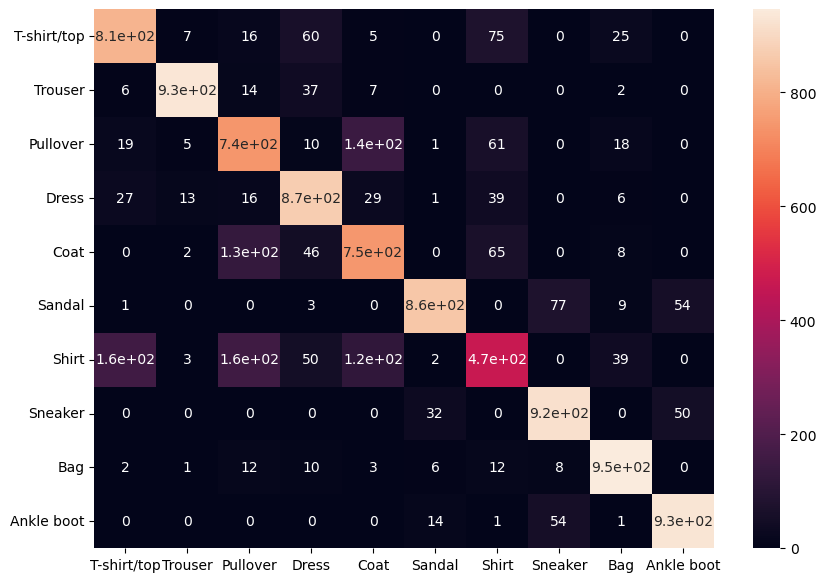
\includegraphics[width=0.65\textwidth]{figures/mlp_no_hidden_cf_fashion.png}
    \caption*{MLP with no hidden layer on FashionMNIST}
\end{figure}

After obtained the above results, my motivations for continuing to test the MLP on these datasets
was more or less squashed. I decided to not fiddle too much with the exact layering structure, layer sizes,
activation functions, etc. as I realized it would be incredibly difficult to notice or attribute any 
performance gains to any of those changes, seeing as the ``null'' model does so well.

\subsection{Radial Basis Function Network}

During the course of this project I wound up spending the most amount of time with RBF Nets
simplying trying to get them to learn the two MNIST datasets.
The implementation that made the most sense to me it shown in the below code chunks,
where I build from the ground up defining an RBF Neruon, then RBF Layer, and finally a full
traditional RBF Net.
However, I had a considerable amount of difficulty getting my implementation to learn anything at all
for the datasets – I was stuck with the RBF Net simply guessing at random.
I went through various levels of debugging first with the individual neruons,
then the entire layer, and lastly the full network, but couldn't find any serious bugs with the
flow through the network.

\begin{lstlisting}[style=Python,caption=RBF Neuron,label=lst:python]
# Single RBF Neuron
class RBFNeuron(nn.Module):

    # mu: RBF mu vector
    # sig: RBF sigma
    def __init__(self, mu, sig):
        super(RBFNeuron, self).__init__()
        self.mu = nn.Parameter(mu)
        self.sig = nn.Parameter(sig)

    def __call__(self, x):
        top = torch.linalg.norm(x-self.mu, dim=1)
        return torch.exp(-0.5*(top / self.sig)**2).float().clone().detach()
\end{lstlisting}

\begin{lstlisting}[style=Python,caption=RBF Layer,label=lst:python]
# Layer of RBF Neurons
class RBFLayer(nn.Module):

    # nin: input dim
    # nout: output dim
    # mus: list of mean vectors for RBF neurons
    # sigs: list of sigmas for RBF neurons
    def __init__(self, nin, nout, mus, sigs):
        super(RBFLayer, self).__init__()
        self.mus = nn.Parameter(mus)
        self.sigs = nn.Parameter(sigs)
        self.neurons = nn.ModuleList([RBFNeuron(mus[i],sigs[i]) for i in range(nout)])

    def __call__(self, x):
        return torch.stack([f(x) for f in self.neurons], dim=1)
\end{lstlisting}

\begin{lstlisting}[style=Python,caption=RBF Network,label=lst:python]
# Full RBF Network
class RBFNet(nn.Module):

    # mus: list of means to use in basis functions
    # sigs: list of sigmas to use in basis functions
    # n_classes: num of classes to pred
    def __init__(self, mus, sigs, n_classes=10):
        super(RBFNet, self).__init__()
        self.K = len(mus) # number of RBFs
        mus = torch.div(mus, torch.linalg.vector_norm(mus, dim=1).view(-1,1)) # unit norm means
        self.mus = nn.Parameter(mus)
        self.sigs = nn.Parameter(sigs)
        self.flatten = nn.Flatten()
        self.layers = nn.Sequential(
            RBFLayer(28*28, self.K, self.mus, self.sigs),
            nn.Linear(self.K, n_classes)
        )

    def forward(self, x):
        x = self.flatten(x)
        x = torch.div(x, torch.linalg.vector_norm(x, dim=1).view(-1,1)) # unit norm x
        return self.layers(x)
\end{lstlisting}

The first step I took was to properly tune $\sigma$ value, since, as mentioned in the
technical description high-dimensional Euclidean space is very sparse, causing a rogue $\sigma$ value
to make the RBF Layer pass through either all 0's or all 1's ruining any chance the netwrok had of learning.
I found it easily enough to tune this manually as I could simply pass some training data through a single 
RBF Neuron with a random cluster center and vary the $\sigma$ until the values looked roughly okay – which
I felt was in the range of $0.1$ to $0.9$.

Once this was handled, I then played with the "basis function" I was using in each neuron since I thought
maybe a non-exponentially decreasing kernel would fix my learning issue, however this really wasn't the case.
I tested a variety of norms as well as some custom kernels I came up with myself, such as $\frac{1}{1+x^2}$ or
$\frac{1}{1+|x|}$, none of which helped the network learn. At this point I was becoming very concerned about my 
implementation even though it looked good. However, I decided to try just passing through the mean of the 
input vector for my "basis function" for some reason, and that wound up allowing the network to learn.
After toying with this for a while I realized that essentially what this was doing was dimensionality reduction
and I may be having a problem with the fact I'm working with a local approximator in a sparse space.

Lastly, I cooked up a simple dataset generator where I could easily vary things like number of clusters,
cluster mean and standard deviation, and most importantly dimensionality. Testing my RBF Net on a simple
few cluster, 2 dimensional dataset shows that it could learn just fine, but as I bumped up the dimensions it 
began to struggle. I found that at around $>$ 25 dimensions it was completely failing to train and would
resort to random guessing. In order to fix this I decided to require everything within or passing through
the network to have a unit norm, with the hopes this would bring all my data points close enough together for
the network to be able to learn a relationship amongst them. Thankfully, this unit norm trick was a success
and allowed enough information to pass through the RBF Layer to train the following Linear layer
(albeit slowly).

I also experimented with first performing K-means clustering then using the cluster centroids as my $\mu$s 
versus simply using training samples as my $\mu$s. For both the MNIST datasets I found this didn't have too much
of an affect on the resulting network performance when using enough basis neurons, though the K-means cluster 
centroids tended to perform slightly better. 
Since the performance was so similar I opted to typically use the training samples themselves.

\subsection{Convolutional Neural Network}

\begin{lstlisting}[style=Python,caption=CNN,label=lst:python]
class CNN(nn.Module):

def __init__(self, kernel_size=3, pool=2, dropout=0.2, n_classes=10):
    super(CNN, self).__init__()
    self.flatten = nn.Flatten()
    self.conv = nn.Sequential(
        nn.Conv2d(in_channels=1, out_channels=8,kernel_size=3, padding=1),
        nn.ReLU(inplace=True),
        nn.MaxPool2d(pool),
        nn.Dropout(dropout),
    )
    self.mlp = nn.Sequential(
        nn.Linear(14*14*8, 64),
        nn.ReLU(inplace = True),
        nn.Dropout(dropout),
        nn.Linear(64, n_classes)
    )
    
def forward(self, x):
    x = self.conv(x)
    x = self.flatten(x)
    return self.mlp(x)
\end{lstlisting}

One of the aspects of working with CNNs I was looking forward to was being able to visualize
the learned filters after training. One interesting paradigm I thought of doing this in was 
after learning a single set of eight $7 \times 7$ filters to see if they would pick up the 
eight types of perimeter features I have in mind that were all 4 corners and all 4 straight edges.
These eight filters are plotted below and just from visual inspection don't seem to all have learned what
might be expected, although some of them (such as the top left) do look to have learned things we might
recognize as important edge features, though for the most part I think they just look like junk.

\begin{figure}[H]
    \centering
    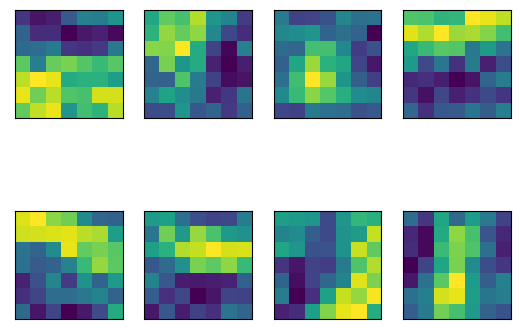
\includegraphics[width=0.9\textwidth]{figures/8filters77.png}
    \caption*{Eight 7x7 Learned DigitMNIST Filters}
\end{figure}

After a somewhat unsuccessful attempt above to get the network to learn what I would think it important
I figured why not see if the network will simply memorize a characteristic example of each digit if 
I let it learn 10 $28 \times 28$ filters. These filters are shown below, and notably some of them do have
a remarkable resemblance to actual digits (I mostly see a 6 and 5 in the top right), although again most
of the filters don't look like anything I'd expect. I then began suspecting that maybe the MLP at the end
of the network was muddying my results, so also visualized the learned filters only using one linear
layer at the end to get down to 10 classes, but this actually made the filters less recognizable.
After all these tests I realized it's most likely that the CNN is using every avenue possible
to learn these digits and instead of allocating each filter to one image it is making use
of it's ability to form linear (or non-linear) combinations of all the filters with the final MLP.

\begin{figure}[H]
    \centering
    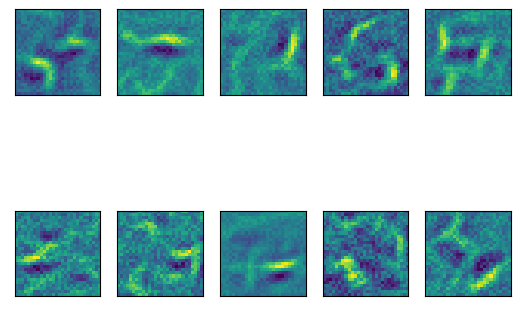
\includegraphics[width=0.9\textwidth]{figures/10filters2828.png}
    \caption*{Ten 28x28 Learned DigitMNIST Filters}
\end{figure}

\subsection{Thoughts and Comparison}

During this project I had a lot of fun with the MLP and CNN, but not so much the RBF.
The only fond memory of the RBF I think I have is when I finally got it to learn something –
anything at all. The MLP and CNN models feel both properly motivated and properly designed to me,
whereas the RBF doesn't make much sense to me from a usability point-of-view.
This is especially magnified when considered how terrible of a time RBFs have with high dimensional
problems – of which there are so many presently. I also think there are some flaws in the standard 
pitch for using RBFs – that is that you may clusters or pick some prototypical examples to use as $\mu$'s in
an RBF layer, then let a linear layer finish everything off. I feel that if you know that much about your 
problem to begin with (e.g., where data is centered at, rough idea of standard deviation, etc.) then
why are you creating a neural network in the first place?

In constrast, I felt that MLP's were nicely motivated (simply multiple layered perceptrons) and also
designed nicely with everything from linear combinations into each neuron, some non-linear activation applied,
then trained via some simple calculus – it just all felt very well-rounded to my mathematical way of thinking.
They also didn't present the issue of required as much data cleaning before being trained or for inference.
I felt similarly about CNNs, as they are a fairly reasonable adjustment to MLPs in the context of
image processing / computer vision.

In terms of performance among the various models, I didn't see enough of a difference during my
other experimentation to feel that it made sense to try and compare them numerically, since for these
MNIST datasets they are all more than capable enough of getting near-perfect results.

\section{Optimization Algorithms}

The last component I wanted to build a better intuiton for was the actual learning algorithms used
to train all these networks. I choose to focus on three that I felt gave a good coverage of how 
cleverly to choose the step size – since that's essentially the only difference between a lot of the
common learning algorithms – SGD, Adagrad, and Adam.

In order to test these learning algorithms I used the below MLP model on FashionMNIST data. I only
ran training for 1 epoch each with a batch size of 4 to see just how much performance these algorithms 
could squeeze out while only seeing the data once. For this problem, the metrics actually point towards
Adagrad being the best optimization algorithm, which I wasn't expecting. I figured that all the 
extra hoops Adam jumped through to determine the ``best'' learning rate would pay off, but at least
in this instance that's not that case as Adam actually looks to have resluted in overfitting.

\begin{lstlisting}[style=Python,caption=MLP model used,label=lst:python]
MLP(
    (flatten): Flatten(start_dim=1, end_dim=-1)
    (layers): Sequential(
        (0): Linear(in_features=784, out_features=512, bias=True)
        (1): ReLU()
        (2): Linear(in_features=512, out_features=512, bias=True)
        (3): ReLU()
        (4): Linear(in_features=512, out_features=10, bias=True)
    )
)
\end{lstlisting}

\begin{table}[h]
    \centering
    \begin{tabular}{|c|c|c|c|c|}
    \hline
    Optimizer & Test Loss & Precision & Recall & F1 Score \\
    \hline
    SGD & 0.5006 & 0.8043 & 0.8043 & 0.8043 \\
    \hline
    Adagrad & 0.0996 & 0.8298 & 0.8298 & 0.8298 \\
    \hline
    Adam & 0.6492 & 0.8144 & 0.8144 & 0.8144 \\
    \hline
    \end{tabular}
    \caption{Optimzer choice influence of metrics}
\end{table}

One oddity I noticed was that all my metrics were essentialy equal (f1 is obviously equal if precision and
recall are). I thought this was possibly a bug but upon further inspection of the confusion matrix it 
makes sense since there are so many data points and the model actually classified roughly the same
amount of false positives and false negatives so the numbers check out.

% Chapter 4: Reflection
\chapter{Reflection}
Would've liked to
- played with more optimization hyperparams
- used some more difficult datasets

% References
\bibliographystyle{plain}
\bibliography{references}


\end{document}
